\documentclass{llncs}
\usepackage{times}
\usepackage[T1]{fontenc}

% Comentar para not MAC Users
% \usepackage[applemac]{inputenc}

\usepackage{a4}
%\usepackage[margin=3cm,nohead]{geometry}
\usepackage{epstopdf}
\usepackage{graphicx}
\usepackage{fancyvrb}
\usepackage{amsmath}
\usepackage[backend=biber]{biblatex}
\addbibresource{references.bib}
%\renewcommand{\baselinestretch}{1.5}

\begin{document}
\mainmatter
\title{Uma pesquisa sobre Software Defined Networking}

\titlerunning{Pesquisa sobre SDN}

\author{Miguel Cruz \and Dinis Peixoto \and João Tomás}

\authorrunning{Miguel \and Dinis \and Tomas}

\institute{
University of Minho, Department of  Informatics, 4710-057 Braga, Portugal\\
e-mail: \{a108574, a108566, a108656\}@alunos.uminho.pt
}

\date{}

\maketitle
\begin{abstract}
    \textit {Software Defined Networking} (SDN) é uma nova abordagem de redes que visa simplificar a sua gestão e permitir a inovação através de redes dinâmicas e programáveis,  revolucionando a arquitetura estática das redes tradicionais, descentralizadas e complexas. 
    O objetivo do SDN é melhorar o controlo da rede, permitindo que as empresas e os fornecedores de serviços respondam rapidamente às mudanças nos requisitos do negócio, possibilitando que um administrador molde o tráfego a partir de uma consola de controlo centralizada sem tocar em switches individuais. Conseguindo alterar as regras de qualquer switch de rede quando necessário – priorizando, despriorizando ou até mesmo bloqueando pacotes específicos com um nível de controlo muito granular.
    Isto é especialmente útil numa arquitetura *multi-inquilino* de \textit {cloud computing}  porque permite ao administrador gerir as cargas de tráfego de forma flexível e mais eficiente.
\end{abstract}

\section{Introdução}

\paragraph{} O crescimento exponencial das *\textit {information and communication technologies} (ICT), particularmente, \textit {cloud computing}, a automação de redes e as redes de \textit {data centers}, é catalisada pela integração de sistemas baseados no SDN. \cite{paper1}
 Com a globalização do digital e o aumento do volume de dispositivos conectados, as arquiteturas de redes tradicionais descentralizadas, que dependem de \textit {hardware} especializado, revelaram-se ineficientes face à necessidade de flexibilidade e de escalabilidade. 
 Neste medida, as redes tradicionais oferecem pouca flexibilidade na gestão do tráfego, bem como incapacidade na resposta às novas exigências computacionais, tais como a baixa latência ou a segmentação de rede. 
 Em contraste, o SDN é uma abordagem inovadora que visa simplificar o tráfego através de redes dinâmicas e programáveis. 
 Com a centralização via \textit {software}, os administradores podem moldar as condições da rede conforme a necessidade, otimizando a utilização de recursos, bem como melhorando a qualidade de serviço (QoS).
 \paragraph{}
Complementarmente, o SDN define-se pelas seguintes características. Primeiramente, a capacidade de desassociar o plano de dados do plano de controlo. \cite{paper3}
 Em segundo lugar, o SDN possui um plano de controlo indefinido, o que permite que seja controlado por um único \textit {software}.
 Por conseguinte, o plano de controlo do SDN estende o seu controlo sobre os elementos do plano de dados da rede, por meio do OpenFlow, programa de interface mais utilizado mundialmente.
 Paralelamente, a arquitetura do SDN providencia que um administrador visione a rede globalmente, mas também que faça alterações globalmente.
 \paragraph{}
Neste trabalho, procuramos apresentar a definição de SDN, bem como a sua arquitetura, aliada aos desenvolvimentos existente à data do SDN, bem como abordagens que visionem o desenvolvimento do SDN.
 O trabalho está organizado da seguinte forma. Na segunda secção, apresentaremos uma definição de SDN, a par dos seus benefícios.
 Nas três secções seguintes, apontaremos prospecções de futuros desenvolvimentos possíveis do SDN. 
 Particularmente, na secção três indicaremos otimizações dos controladores SDN, já a secção quatro demonstra um sistema híbrido do SDN e as \textit {legacy networks}, e a secção cinco exibe o desempenho do SDN em larga escala, bem como a sua prospecção face às otimizações mencionadas anteriormente. 
 E, uma sucinta conclusão, que engloba o as implementações atuais do SDN, mas também uma antevisão das implementações futuras, e dos seus benefícios, na secção seis.
 \paragraph{}
\section{SDN: definição e benefícios}
\paragraph{}
Devido à sua emergência, o SDN ainda não dispõe uma definição consensual.
Nesta secção, iremos primeiramente apresentar a mais definição mais creditada, e posteriormente, os benefícios do SDN.

\subsection{Definição de SDN}
\paragraph{}
De acordo com a Open Networking Foundation (ONF), \textit{Software Defined Networking} (SDN) é uma arquitetura de redes dinámica, controlável, econômica e flexível, tornando-a ideal para os usos de banda larga das aplicações atuais. 
Esta arquitetura desassocia as funções de controlo e encaminhamento da rede, possiblitando que o controlo da rede seja diretamente programável. \cite{fundation2012software}
\paragraph{}
Convergentemente, o ONF dispõe de um modelo de referẽncia do SDN, como ilustrado na figura \ref{fig:architecture}
\begin{figure}
\begin{center}
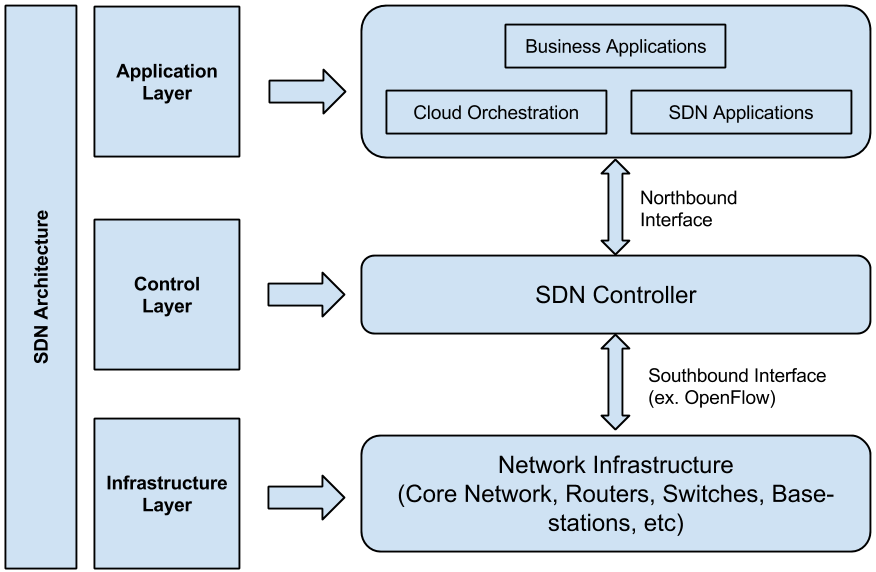
\includegraphics[scale=0.40]{figura1.png} 
\end{center}
\caption{\label{fig:architecture}Modelo de Referência do SDN, segundo a ONF.}
\end{figure} 
\paragraph{}

A camada de infraestrutura consiste em dispositivos de comutação (por exemplo, \textit{switches}, \textit{routers}, etc.) no plano de dados.
As funções destes dispositivos de comutação são basicamente duplas. 
Primeiro, são responsáveis ​​por recolher o estado da rede, armazená-los temporariamente em dispositivos locais e enviá-los para os controladores. 
O estado da rede pode incluir informações como a topologia da rede, estatísticas de tráfego e utilizações da rede. 
Em segundo lugar, são responsáveis ​​pelo processamento de pacotes com base em regras fornecidas por um controlador.
\paragraph{}
A camada de controlo faz a ponte entre a camada de aplicação e a camada de infraestrutura, através das suas duas interfaces. Para a interação descendente com a camada de infraestrutura (ou seja, a interface virada a sul), especifica funções para os controladores acederem a funções fornecidas pelos dispositivos de comutação. As funções podem incluir relatórios do estado da rede e importação de regras de encaminhamento de pacotes. Para uma interação ascendente com a camada de aplicação (ou seja, a interface norte), fornece pontos de acesso de serviço em várias formas, por exemplo, uma \textit{Application Programming Interface} (API). As aplicações SDN podem aceder a informações de estado de rede reportadas a partir de dispositivos de comutação através desta API, tomar decisões de ajuste do sistema com base nessas informações e executar essas decisões configurando regras de encaminhamento de pacotes para dispositivos de comutação utilizando esta API. Como existirão múltiplos controladores para um grande domínio administrativo de rede, uma interface de comunicação “leste-oeste” entre controladores também exigirá que os controladores partilhem informações de rede e coordenem os seus processos de tomada de decisão.
\paragraph{}
A camada de aplicação contém aplicações SDN concebidas para satisfazer os requisitos do utilizador. Através da plataforma programável fornecida pela camada de controlo, as aplicações SDN são capazes de aceder e controlar dispositivos de comutação na camada de infraestrutura. Exemplos de aplicações SDN podem incluir o controlo de acesso dinâmico, o balanceamento de carga do servidor e a virtualização de rede.

\subsection{Benefícios do SDN}

\section{Optimização de controladores SDN}

\section{Integração de SDN com \textit{legacy networks}}
\paragraph{}
Um problema do OpenFlow é a utilização de redes virtualizadas, que é uma ferramenta essencial para os ambientes de experimentação.
À semelhança da virtualização, procura melhorar a alocação de recursos permitindo aos operadores criar pontos de verificação para a sua rede antes de fazer alterações, e garante que os clientes concorrentes possam partilhar os mesmos equipamentos de forma controlada e isolada. 
Permite ainda que um conjunto de \textit{switches} seja partilhado entre múltiplas redes lógicas, cada uma com a mesma lógica de encaminhamento distinta e utilizando o mesmo plano de encaminhamento de \textit{hardware}, que são hoje as principais características dos ambientes \textit{Future Internet} (FI).
\paragraph{}
No entanto, hoje em dia tanto as instalações de experimentação de FI como as redes OpenFlow enfrentam um grande desafio: como podem integrar estes ambientes com ambientes de rede híbrida (i.e., OpenFlow e Legacy Network)? 
Inicialmente é necessário conceptualizar Rede Legada, são redes com equipamentos utilizados por não-OpenFlow (e.g. a actual rede Internet) ou tecnologias que não são suportadas pelo OpenFlow (e.g. tecnologias de circuitos Camada 1 e Camada 0). 
Alguns dos desafios das redes OpenFlow estão relacionados com a compatibilidade e os requisitos de integração com ambientes de \textit{legacy networks}.
\paragraph{}
Outra questão, o OpenFlow não é capaz de manipular ou gerir equipamentos de legado pelo protocolo OpenFlow e, como resultado, é extremamente difícil alocar recursos em redes legadas para ligar dois ambientes OpenFlow. 
Para além de outros problemas que surgem durante a implementação, existe um problema prático que envolve \textit{ legacy switches} que não suportam o protocolo OpenFlow e precisam de ser substituídos ou atualizados.

\section{Desempenho em implementações em larga escala}
\paragraph{}
Podemos dizer que as tecnologias e protocolos habilitadas pelo SDN contribuem significativamente para o sucesso do \textit {cloud computing}, bem como para a automação de redes e \textit {data centers}. O SDN permite satisfazer os requirementos de recursos \textit{on demand} dos utilizadores na \textit{cloud}. 
É uma infraestrutura inovadora que consegue preencher a lacuna entre as redes convencionais de \textit{data centers} e os requesitos computacionais e de armazenamento dos utilizadores.
O SDN consegue superar as tecnologias de redes existentes, oferecendo serviços extra oferecendo vários serviços sem esforços extra e despesas gerais a um custo mínimo, como gestão de rede consolidada, segurança de rede robusta, escalabilidade, adaptabilidade, estratégias de \textit {backtesting} mais seguras, unificação perfeita de recursos de \textit{cloud} e entrega garantida de conteúdo.


%UNCOMMENT se necess�rio
%De acordo com o ilustrado na Figura~\ref{fig:controller}
%% Exemplo para inser��o de uma figura
%\begin{figure}
%\begin{center}
%\includegraphics[scale=0.40]{figura.pdf} 
%\end{center}
%\caption{\label{fig:controller}Architecture of the unified QoS metric fuzzy controller.}
%\end{figure} 

%According to Table~\ref{tab:TabelaExemplo}...

% Exemplo de uma tabela com duas colunas
%\begin{figure}
%\centering
%\begin{tabular}{|c|c|}\hline
%(a) Delay and jiiter & (b) Delay and loss \\ \hline

%(c) Delay and throughput & (d) Jitter and loss \\ \hline

%(e) Jitter and throughput & (f) Loss and throughput \\ \hline
%\end{tabular}
%\caption{\label{tab:TabelaExemplo}Tabela exemplo.}
%\end{figure}

%\section{Simulation Scenario}

\section{Conclusões}
\paragraph{}
Neste trabalho...

\printbibliography

\end{document}